\chapter{Klassifikation}

Klassifikation bezeichnet Algorithmen im Bereich des \emph{supervised
Learnings}, welche Datenpunkte anhand bekannter Klassenlabels in vordefinierte
Kategorien einordnen. Ziel ist, auf Basis eines Trainingsdatensatzes mit
Features und zugehörigen Labels ein Modell zu lernen, das für neue, unbekannte
Datenpunkte möglichst korrekte Vorhersagen trifft. Gute Klassifikatoren
zeichnen sich durch hohe Treffergenauigkeit (Accuracy), gute Trennung
zwischen den Klassen (Precision/Recall, AUC) und robuste Leistung bei
unterschiedlichen Klassenhäufigkeiten aus (vgl \cite{Miller2024}).

Viele dieser Metriken basieren im binären Fall auf den vier Kategorien einer
\emph{Konfusionsmatrix} (\ac{TP}, \ac{FP}, \ac{TN}, \ac{FN})
(vgl. Abbildung~\ref{fig:confmat}). Im folgenden Beispiel wurden von 100 Instanzen
insgesamt 30 als \textbf{True Positives}, 10 als \textbf{False Positives}, 15 als \textbf{False Negatives}
und 45 als \textbf{True Negatives} klassifiziert. Dieses Beispiel wird im Folgenden zur als Beispiel
der Berechnung einzelner Metriken genutzt.
Ein komplexeres Beispiel, in welchen Algorithmen auf einen Brustkrebsdatensatz trainiert wurden und bestimmen sollen ob der 
Brustkrebs bösartig oder gutartig ist, ist im verlinkten GitHub-Repository zu finden.

\begin{figure}[ht]
  \centering
  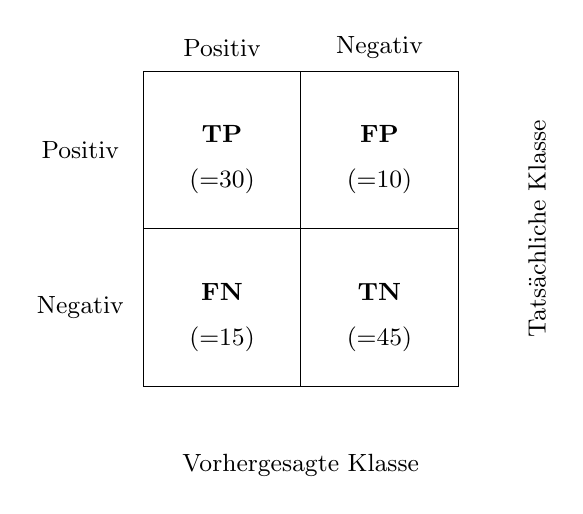
\begin{tikzpicture}[font=\small]
    % Gitter und Linien
    \draw (0,0) rectangle (4,4);
    \draw (2,0) -- (2,4); % vertikale Mittellinie
    \draw (0,2) -- (4,2); % horizontale Mittellinie

    % Boxenbeschriftung + Beispielwerte
    \node at (1,3.2) {\textbf{TP}};
    \node at (1,2.6) {(=30)};
    
    \node at (3,3.2) {\textbf{FP}};
    \node at (3,2.6) {(=10)};
    
    \node at (1,1.2) {\textbf{FN}};
    \node at (1,0.6) {(=15)};
    
    \node at (3,1.2) {\textbf{TN}};
    \node at (3,0.6) {(=45)};

    % Achsenbeschriftung
    \node[rotate=90] at (5,2) {Tatsächliche Klasse};
    \node at (2,-1) {Vorhergesagte Klasse};

    % Spaltenbeschriftung (Predicted)
    \node at (1,4.3) {Positiv};
    \node at (3,4.3) {Negativ};

    % Zeilenbeschriftung (Actual)
    \node at (-0.8,3) {Positiv};
    \node at (-0.8,1) {Negativ};
  \end{tikzpicture}
  \caption{Konfusionsmatrix mit Beispielwerten}
  \label{fig:confmat}
\end{figure}

\section{Accuracy (Treffergenauigkeit)}
Die Accuracy misst den Anteil korrekt klassifizierter Instanzen an allen Fällen.  
\[
\mathrm{Accuracy}=\frac{TP+TN}{TP+FP+FN+TN} = \frac{30+45}{100} = 0{,}75
\]
Somit misst sie wie viele Vorhersagen insgesamt richtig waren.
Eine hohe Accuracy ist nur aussagekräftig, wenn die Klassenverteilung ausgeglichen ist (vgl. \cite{Miller2024}).

\section{Precision, Recall, F1-Score}
Diese drei Metriken sind besonders wichtig, wenn die Klassenverteilung unausgeglichen ist (z.\,B. bei seltenen Ereignissen)(vgl. \cite{powers2020evaluation} S.38f).

\textbf{Precision} (Positiver Vorhersagewert):
\[
\mathrm{Precision} = \frac{TP}{TP+FP} = \frac{30}{30+10} = 0{,}75
\]
Precision beschreibt den Anteil der als positiv vorhergesagten Fälle, die tatsächlich positiv sind.  
Somit sollte diese Metrik verwendet werden, wenn \ac{FP} teuer sind (z.\,B. Spam‑Filter).  
Allerdings wird ignoriert, wie viele echte Positive verpasst werden.

\textbf{Recall} (Sensitivität, Trefferquote):
\[
\mathrm{Recall} = \frac{TP}{TP+FN} = \frac{30}{30+15} = 0{,}67
\]
Recall beschreibt den Anteil der tatsächlichen Positiven, die korrekt erkannt wurden.  
Die Metrik ist somit relevant, wenn \ac{FN} kritisch sind (z.\,B. Krebsdiagnose).  

\textbf{F\(_1\)-Score} (harmonisches Mittel):
\[
F_1 = 2 \cdot \frac{\mathrm{Precision}\,\times\,\mathrm{Recall}}{\mathrm{Precision} + \mathrm{Recall}}
\approx 0{,}71
\]
Der F1-Score balanciert Precision und Recall und gibt nur dann hohe Werte, wenn beide hoch sind.  
Beachtet allerdings \ac{TN} nicht und ist daher nicht vollständig aussagekräftig, wenn TN wichtig sind (vgl. \cite{powers2020evaluation} S38f).

\section{ROC-Kurve und AUC (Area Under the Curve)}
Die \ac{ROC}-Kurve ist ein Werkzeug zur Bewertung von binären
Klassifikationsmodellen. Sie zeigt den Zusammenhang zwischen der \emph{True
Positive Rate} (Recall) und der \emph{False Positive Rate} (FPR) für
verschiedene Entscheidungs­schwellen (Thresholds) des Modells.

\begin{align*}
\mathrm{TPR} &= \frac{TP}{TP + FN} \quad \text{(Recall)} \\
\mathrm{FPR} &= \frac{FP}{FP + TN}
\end{align*}

\textbf{Interpretation:}  
Die \ac{ROC}-Kurve zeigt, wie gut ein Modell zwischen den Klassen unterscheidet. Sie
beginnt immer bei (0,0) und endet bei (1,1). Je näher die Kurve an der oberen
linken Ecke liegt, desto besser ist das Modell (vgl. \cite{Miller2024}).

\ac{AUC} ist die Fläche unter der ROC-Kurve:
\begin{itemize}
  \item AUC = 1: perfekter Klassifikator
  \item AUC = 0.5: reines Raten (Zufall)
  \item AUC < 0.5: systematisch falsche Klassifikation
\end{itemize}

\textbf{Vorteile:}  
AUC ist unabhängig vom gewählten Schwellenwert und eignet sich besonders bei unausgeglichenen Klassenverhältnissen.

\begin{figure}[ht]
  \centering
  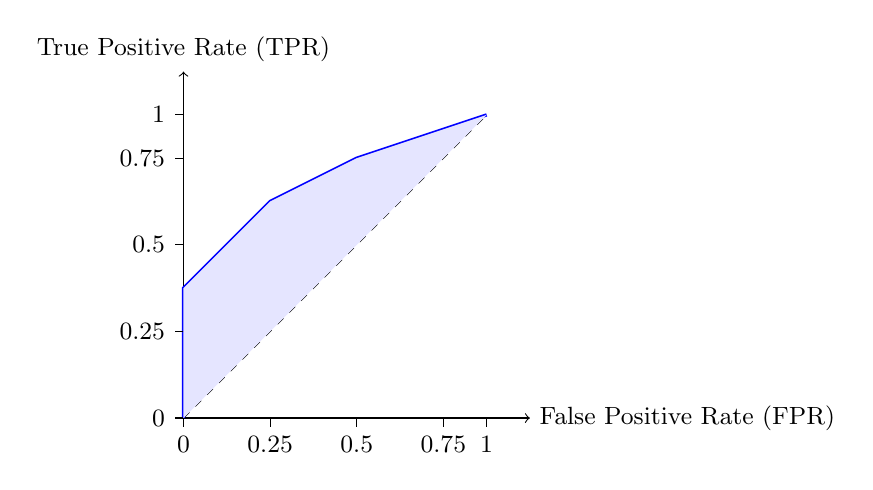
\begin{tikzpicture}[scale=1.1, font=\small]
    % Achsen
    \draw[->] (0,0) -- (4,0) node[right] {False Positive Rate (FPR)};
    \draw[->] (0,0) -- (0,4) node[above] {True Positive Rate (TPR)};

    % Diagonale
    \draw[dashed] (0,0) -- (3.5,3.5);

    % Beispiel ROC-Kurve
    \draw[very thick, blue] 
      (0,0) -- (0,1.5) -- (1,2.5) -- (2,3) -- (3.5,3.5);

    % Fläche unter Kurve (schematisch)
    \fill[blue!10] 
      (0,0) -- (0,1.5) -- (1,2.5) -- (2,3) -- (3.5,3.5) -- (0,0);

    % Markierungen
    \foreach \i/\label in {0/0, 1/0.25, 2/0.5, 3/0.75}
      {
        \draw (\i,0) -- (\i,-0.1) node[below] {\label};
        \draw (0,\i) -- (-0.1,\i) node[left] {\label};
      }
    \draw (3.5,0) -- (3.5,-0.1) node[below] {1};
    \draw (0,3.5) -- (-0.1,3.5) node[left] {1};

  \end{tikzpicture}
  \caption{Beispielhafte ROC-Kurve (blau) und zufälliger Klassifikator (gestrichelt)}
  \label{fig:roc}
\end{figure}

\textbf{Beispiel:}  
Angenommen, ein Modell trifft mit variabler Schwelle folgende Entscheidungen (sortiert nach Modell-Score):

\begin{center}
\begin{tabular}{|c|c|c|}
\hline
Score & Wahre Klasse & Klassifikation bei Schwelle \\
\hline
0.9 & Positiv & Positiv \\
0.8 & Negativ & Positiv \\
0.7 & Positiv & Positiv \\
0.4 & Positiv & Negativ \\
0.2 & Negativ & Negativ \\
\hline
\end{tabular}
\end{center}

Bei Variation der Schwelle kann man verschiedene (FPR, TPR)-Punkte erzeugen und so die ROC-Kurve aufbauen (siehe Abbildung \ref{fig:roc}).

\section{Mehrklassige Klassifikation}

Zur Evaluation nicht‑binärer Klassifikationsprobleme lassen sich die Evaluationsmetriken über alle Klassen hinweg zusammenfassen.
Hierbei gibt es zwei Ansätze (vgl. \cite{takahashi2022confidence}):

\begin{itemize}
  \item \textbf{Micro-Averaging}:  
    \begin{itemize}
      \item Man fasst alle Klassen‑Confusion‑Matrix‑Einträge instanzübergreifend zusammen:
      \[
        TP = \sum_{i=1}^r TP_i,\quad
        FP = \sum_{i=1}^r FP_i,\quad
        FN = \sum_{i=1}^r FN_i.
      \]
      \item Anschließend werden die Metriken wie im binären Fall berechnet.
    \end{itemize}

  \item \textbf{Macro-Averaging}:  
    \begin{itemize}
      \item Für jede Klasse \(i\) separat:
      \[
        P_i = \frac{TP_i}{TP_i + FP_i},\quad
        R_i = \frac{TP_i}{TP_i + FN_i},\quad
      \]
      \[
        F_{1,i} = 2\,\frac{P_i\,R_i}{P_i + R_i}.
      \]
      \item Die \emph{Macro-F\(_1\)} ist der einfache Mittelwert:
      \[
        \mathrm{F}_{1,\text{macro}}
        = \frac{1}{r} \sum_{i=1}^r F_{1,i}.
      \]
    \end{itemize}
\end{itemize}

Zusammengefasst gilt für die beiden Metriken:
\begin{itemize}
  \item \textbf{Micro-F\(_1\)}: Gesamtüberblick, instanzgewichtet, robust bei Klassenungleichgewicht.
  \item \textbf{Macro-F\(_1\)}: Klassen gleichgewichtet, macht Schwächen seltener Klassen sichtbar.
\end{itemize}
